% Introduction


\section{Introduction}


\begin{figure}
    \centering
    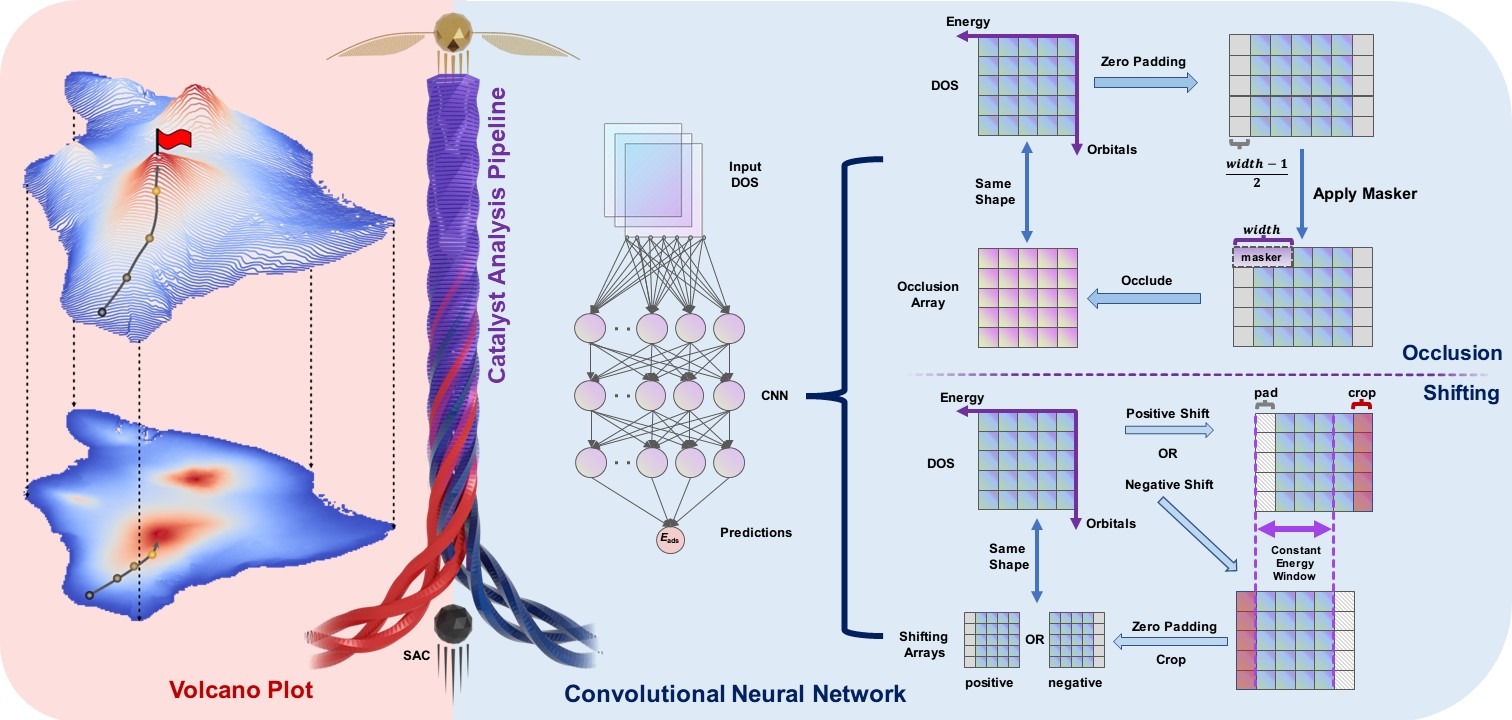
\includegraphics[width=0.95\linewidth]{main_sections/figures/main_fig1_pipeline.JPG}
    \caption{\textbf{Catalyst Performance Analysis Pipeline Integrating Volcano Plots and CNN.}
    The figure demonstrates the integrated usage of volcano plots for predictive assessments of existing catalysts and the utility of CNNs to predict and modulate adsorption energies \(E_{\text{ads}}\) using eDOS as input.
    Advanced occlusion and shifting experiments on eDOS are conducted to extract chemical meanings from CNN model.}
    \label{main_fig1:pipeline}
\end{figure}


Electrochemical CO$_2$RR stands as a promising avenue for long-term seasonal energy storage \cite{dinh2018co2} and mitigating excess CO$_2$ in the atmosphere.

Despite decades of research, metallic copper remains a leading CO$_2$RR electrocatalyst for hydrocarbon production \cite{osella2023co2}, albeit burdened by substantial overpotential and low faradic efficiency and poor operational stability \cite{chen2019identifying, liu2021co2}.
In this regard, supported SACs have displayed remarkable activity and selectivity across various catalytic reactions \cite{wang2018heterogeneous, yang2018atomically}, leveraging their unique electronic properties and coordination environment.
To date, experimental studies have primarily focused on two-electron reduction products due to the facile release of gaseous CO \cite{cai2021insights, ju2017understanding, ren2019isolated}.
Consequently, there is a pressing need to modulate the electronic structure of single-atom sites to enable hydrocarbon production at reduced overpotential.

The challenge towards effective catalysts design lies in understanding the reaction mechanisms.
Experimental determination of these mechanisms remains challenging due to the complexity of in situ spectroscopic detection of reaction intermediates \cite{zhao2021revisiting}.
Computational modeling, particularly methods based on quantum mechanics (QM) such as density functional theory (DFT),
allows for the profiling the energetics of intermediates and unveils structure-activity relationships for identified active sites \cite{feaster2017understanding, carter2008challenges}, contributing to understanding of reaction mechanisms.
However, the high computational cost of QM methods restricts the accessible catalyst space \cite{jinnouchi2017predicting, cuenya2015nanocatalysis, goldsmith2018machine}.

In this context, researchers have explored descriptor-based methods to circumvent QM calculations and establish direct correlations between target properties and electronic factors, commonly referred to as descriptors or features.
Traditional methods of crafting descriptors, as seen in the d-band model of Hammer and Nørskov \cite{hammer1995electronic}, necessitate meticulous selection of chemical properties based on chemical knowledge and are inherently case-dependent \cite{kajita2017universal}.
Particularly in the case of SACs, the relationship is intricate, rendering manual crafting inadequate \cite{han2021single, thirumalai2018investigating}.
To streamline this featurization process, we employed convolutional neural networks (CNNs), which autonomously derive a hierarchical representation directly from the electronic density of state (eDOS) \cite{tran2015learning, socher2012convolutional, krizhevsky2012imagenet}.
This approach accurately maps to the activity space, negating the need for manual crafting of descriptors and providing a more efficient method to understand and establish the structure-mechanism-activity relationship for electrochemical reactions.

In this study, we introduced a catalyst performance analysis pipeline (\cref{main_fig1:pipeline}) integrating a customized CNN model and volcano plots.
Our CNN model accurately estimated the adsorption energies, the activity descriptor, from the eDOS of 2D materials supported single metal catalysts.
Evaluations on the adsorption energies of nine intermediates along CO$_2$RR and competing hydrogen evolution reaction (HER) as well yielded prediction mean absolute errors (MAEs) at the level of 0.1 eV, which is well aligned with the precision of conventional DFT calculations \cite{kirklin2015open, lejaeghere2016reproducibility, wellendorff2015benchmark}.
This result validated the capability of current CNN model to accurately capture intricate spatial information from eDOS.
Building on this, we introduced an orbitalwise eDOS occlusion experiment was adopted afterwards inspired from the occlusion technique widely used in computer vision and pattern recognition applications.
Systematic eDOS experiment was performed to elucidate orbitalwise contributions to the adsorption energies at different energy levels, which produced consistent outcome from Crystal Orbital Hamilton Population (COHP) analysis and real-space wavefunction visualization.
All these results justified the proficiency of CNN model on identifying the dominant orbitals for adsorbate-substrate interactions.
Furthermore, orbital-wise eDOS shifting experiment, exploring the impact of orbital-wise eDOS shifting on the adsorption behavior of studied catalysts were performed.

Simultaneously, we incorporated the volcano plots into the catalysis performance analysis pipeline.
Besides offering intuitive analysis of catalyst activities (represented by the elevation of volcanoes), volcano plots points to the directions on how effort can be exerted to identify promising catalyst candidates.
Built upon scaling relations \cite{peterson2012activity}, we introduced a hybrid-descriptor scheme incorporating both C- and O-centered species.
The scaling coefficient of determination ($R^2$) was increased by 0.1387 using hybrid descriptor, which demonstrate an improved prediction accuracy compared to the well documented single descriptor based method.

In summary, we introduced a catalyst performance analysis pipeline by integrating CNN and volcano plot analysis, using CO$_2$RR as an example proof of concept.
The CNN, which correlates eDOS with activity descriptors, establishes a robust electronic structure-activity relationship.
Notably, it is capable to predict the influence of eDOS disturbances, caused by either alloying, strain, or defects \cite{norskov2011density, bera2017density, kusada2019emergence}, to modulate the catalytic activity of materials, which will offer insights into the intrinsic mechanism for rationalized catalyst optimization strategies.
Advancing the current volcano plot method, the involvement of CNN models in catalyst performance analysis pipeline holds enormous promise for advanced exploration of catalysts with superior performance.
